%
\section{Motivating Examples}\label{sec mot}
%\newpage
%\newpage
% (Chang, Lizzie please fill here)
%\subsection{Verifying Analytical Predictions}

\begin{figure}[t!]
	\begin{subfigure}{1.5in}\vspace{-5pt}
		\centering
		\begin{tikzpicture}
		\node at (0,0) {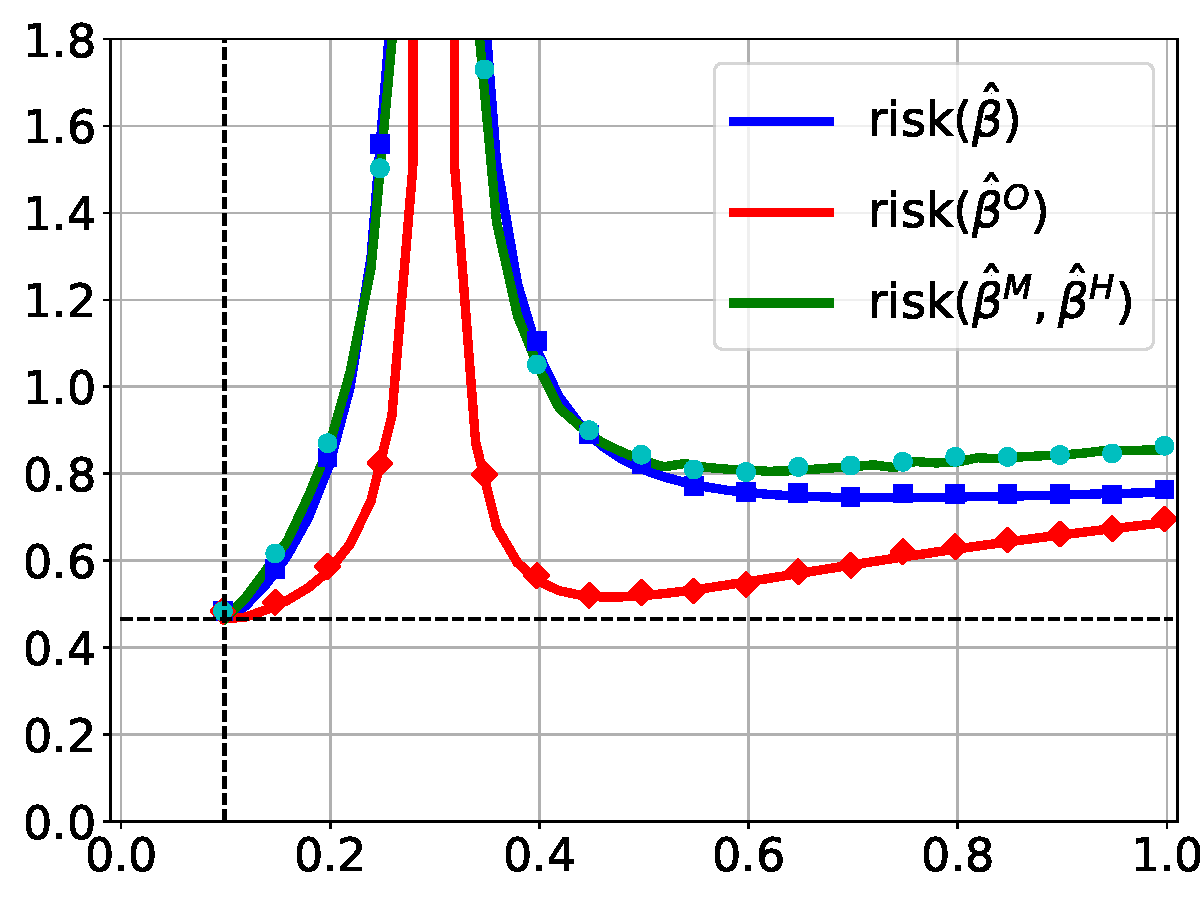
\includegraphics[scale=0.2]{figs/FLAT_SIM_s10_n30_p100_SCL25}};
		\node at (-2.1,0) [rotate=90,scale=.9]{Test Risk};
		\node at (0,-1.7) [scale=.9]{Problem Size ($k/p$)};%Each bar in the figure shows the correlations' geometric mean of datasets in this group when training to corresponding non-zero level. 
		\end{tikzpicture}\caption{\small{Identity covariance, spiked latent weights.}}\label{fig1a}\vspace{-0.2cm}
	\end{subfigure}~~~~~\begin{subfigure}{1.5in}\vspace{-5pt}
	\centering
	\begin{tikzpicture}
	\node at (0,0) {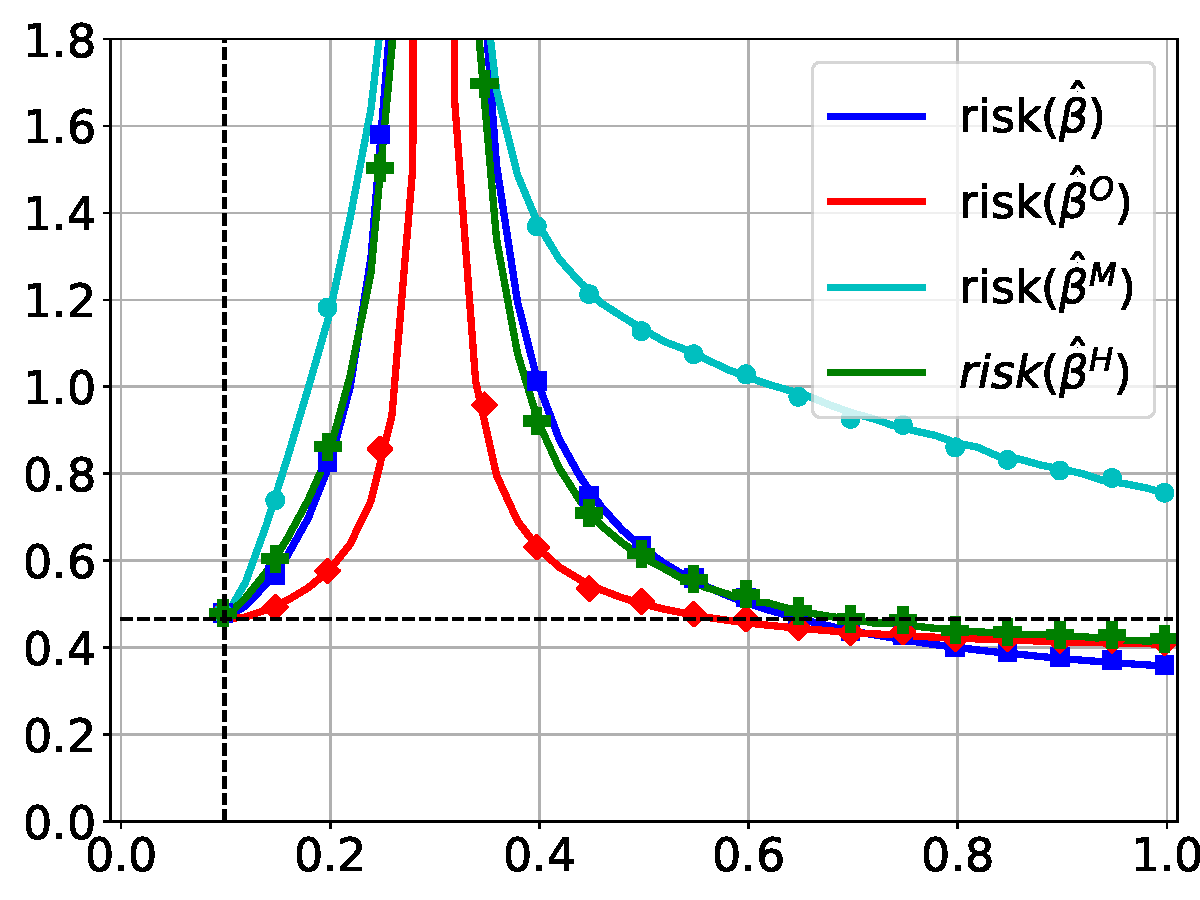
\includegraphics[scale=0.2]{figs/SPIKE_SIM_s10_n30_p100_SCL25}};
	%\node at (-2.4,0) [rotate=90,scale=1.]{Test Risk};
	\node at (0,-1.7) [scale=.9]{Problem Size ($k/p$)};%Each bar in the figure shows the correlations' geometric mean of datasets in this group when training to corresponding non-zero level. 
	\end{tikzpicture}\caption{\small{Spiked covariance, identical latent weights.}}\label{fig1b}\vspace{-0.2cm}
\end{subfigure}\caption{\small{Our theoretical predictions for various pruning strategies in linear models with $s/p=0.1$ and $n/p=0.3$. We solve ERM using the first $k$ features and then prune to obtain an $s$-sparse model. The vertical dashed line shows the $k=s$ point. The horizontal dashed line highlights the minimum risk among all underparameterized solutions ($k\leq n$) and all solutions obtained by a final retraining. \fy{Retraining curves are omitted here, but they can be found in Fig.~7 of SM.}}}\label{fig1}\vspace{-15pt}
\end{figure}
% and oracle pruning

%\begin{figure}[t!]
%	\begin{subfigure}{1.5in}\vspace{-5pt}
%		\centering
%		\begin{tikzpicture}
%		\node at (0,0) {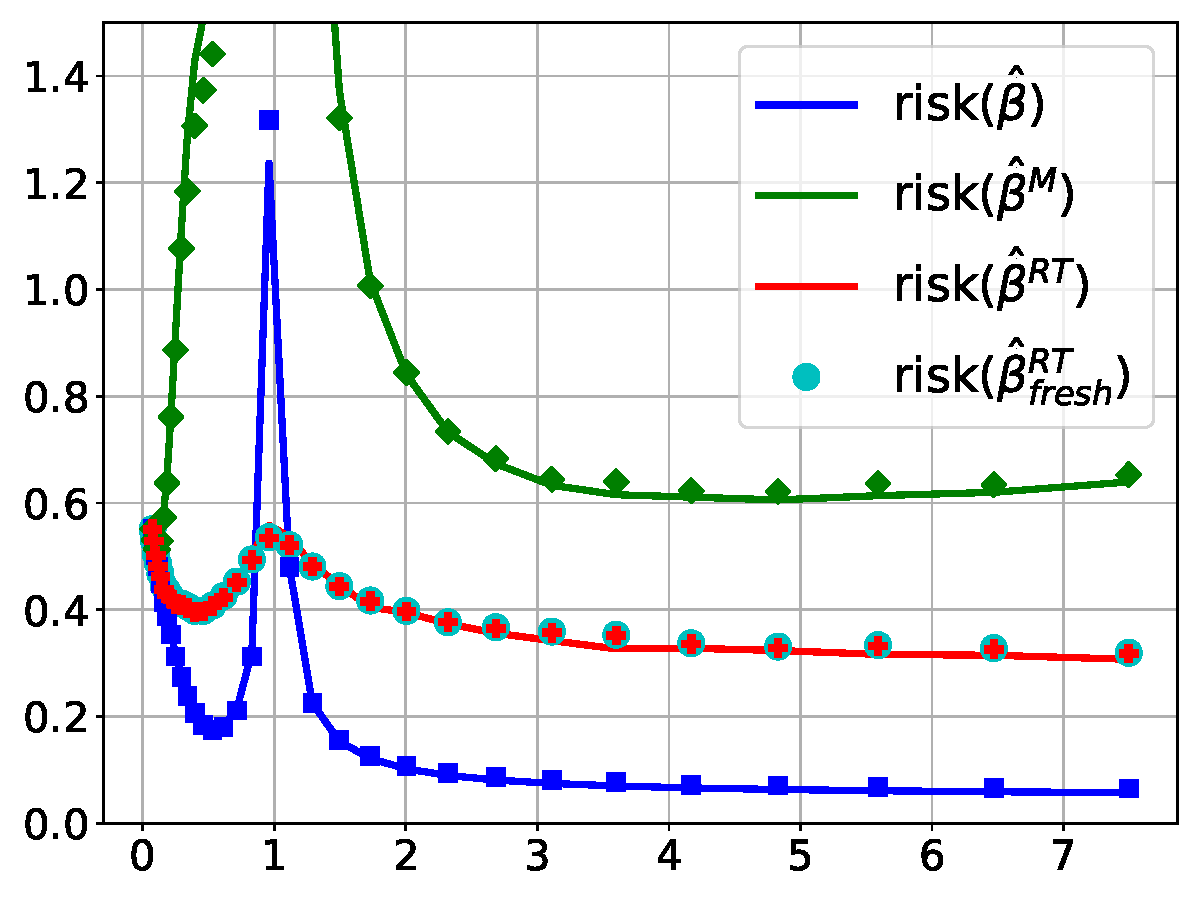
\includegraphics[scale=0.18]{figs/RF_SIM_s15_n200_p1500}};
%		\node at (-1.9,0) [rotate=90,scale=.9]{Test Risk};
%		\node at (0,-1.5) [scale=.9]{Problem Size ($k/p$)};%Each bar in the figure shows the correlations' geometric mean of datasets in this group when training to corresponding non-zero level. 
%		\end{tikzpicture}\caption{\small{Identity covariance, variable weight magnitudes.}}\label{fig1a}\vspace{-0.2cm}
%	\end{subfigure}~\begin{subfigure}{1.5in}\vspace{-5pt}
%	\centering
%	\begin{tikzpicture}
%	\node at (0,0) {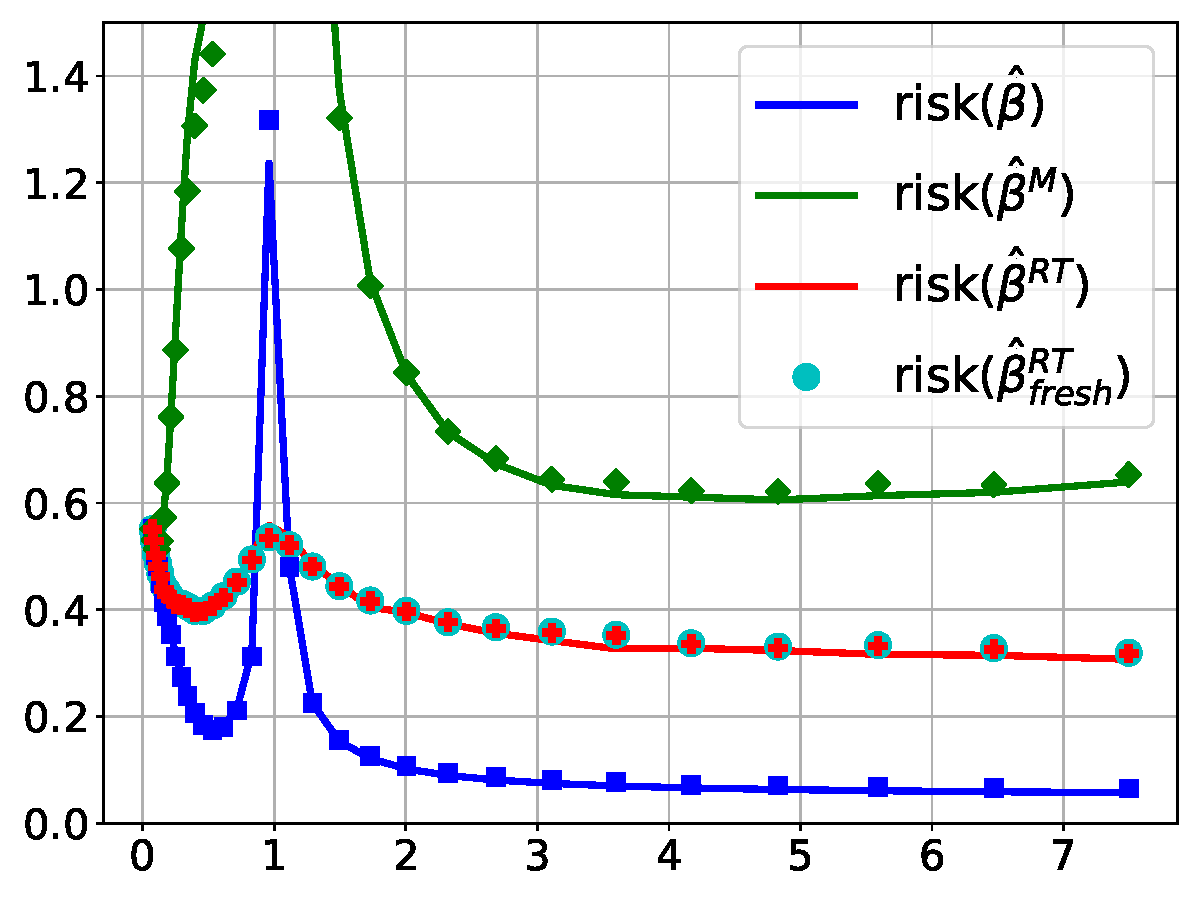
\includegraphics[scale=0.18]{figs/RF_SIM_s15_n200_p1500}};
%	%\node at (-2.4,0) [rotate=90,scale=1.]{Test Risk};
%	\node at (0,-1.5) [scale=.9]{Problem Size ($k/p$)};%Each bar in the figure shows the correlations' geometric mean of datasets in this group when training to corresponding non-zero level. 
%	\end{tikzpicture}\caption{\small{Variable covariance, identical weight magnitudes.}}\label{fig1b}\vspace{-0.2cm}
%\end{subfigure}\caption{\small{Dashed line denotes the $k=s$ point.}}\label{fig1}\vspace{-15pt}
%\end{figure}


%When covariance $\bSi$ is diagonal, for population loss, it can be shown that the saliency of $i$th feature is equal to $\bSi_{i,i}\bt_i^2$ which motivates Hessian pruning. 
%In our experiments, we fix the latent saliency scores to a vector $\bla\in\R^p$ i.e.~we set $\bla_i=\bSi_{i,i}\bt_i^2$. 
%This means that the first $s$ entries have larger saliency than the remaining $p-s$. 
%Additionally, we also visualize, what we call, the oracle pruning $\bth^O_s([k])$ which knows the location of the salient features and always chooses the first $s$ nonzeros of $\bth([k])$. 
%\noindent \textbf



%\subsection{Linear Problem with Uncorrelated Features} 
\subsection{Linear Gaussian Problems} 
We begin our study with linear Gaussian problems (LGP), which we formally define as follows. 
\begin{definition}[Linear Gaussian Problem (LGP)] \label{def LGP}Given latent vector $\bt^\st\in\R^d$, covariance $\bSi$ and noise level $\sigma$, assume that each example in $\Sc$ is generated independently as $y_i=\x_i^T\bt^\st+ \sigma z_i$ where $z_i\sim\Nn(0,1)$ and $\x_i\sim\Nn(0,\bSi)$. Additionally, the map $\phi(\cdot)$ is identity and $p=d$.
\end{definition}
Albeit simple, LGPs are of fundamental importance for the following reasons: (1) We show in Sec. \ref{sec main} that our theoretical framework rigorously characterizes pruning strategies for LGPs; (2) Through a ``linear Gaussian equivalence", we will use our results for linear models to obtain analytic predictions for nonlinear random features; (3) Our theoretical predictions and numerical experiments discussed next demonstrate that LGPs already capture key phenomena observed in more complex models (e.g., Fig. \ref{figNN}).
%. Moreover, 
%We first start with LGP experiments that are perfectly characterized within our theoretical framework. 

In Fig.~\ref{fig1}, we consider LGPs with diagonal covariance $\bSi$. We set  the sparsity  level $s/p=0.1$ and the relative dataset size $n/p=0.3$. To parameterize the covariance and $\bt^\st$, we use a {\em{spiked}} vector $\bla$, the first $s$ entries of which are set equal to $C=25\gg 1$ and the remaining entries equal to $1$. $\bla$ corresponds to the latent saliency score (cf. ~\eqref{saliency eq}) of the indices. To understand the role of overparameterization, we vary the number of features used in the optimization. Specifically, we solve \eqref{eq:ERM} with $\Delta=[k]$ and vary the number of features $k$ from $0$ to $p$. Here we consider the {\em{train$\rightarrow$prune}} algorithm, where we first solve for $\bth([k])$ and obtain our pruned model $\bth^P_s([k])$ by applying magnitude, Hessian or Oracle pruning (cf. ~$P\in \{M,H,O\}$). Since $\bla$ is non-increasing, the indices are sorted by saliency score; thus, Oracle pruning always picks the first $s$ indices. Solid lines represent analytic predictions, while markers are empirical results.
 %Our theoretical predictions and empirical results are shown in Fig.~\ref{fig1}, with simplified notation $\bth^P_s([k])\rightarrow \bth^P$. 
 The vertical dashed line is the sparsity level $s/p$. 

\cmt{confusing about why setups of Fig.~\ref{fig1a}, \ref{fig1b}. Are we trying to keep saliency score the same?}
In Fig.~\ref{fig1a}, we set $\bSi=\Iden_p$ and $\bt^\st=\sqrt{\bla}$. Note, that the analytic curves correctly predict the test risk and the double descent behavior. Observe that the Hessian and Magnitude pruning coincide here, since the diagonal of the empirical covariance is essentially identity. In contrast, Fig.~\ref{fig1b} emphasizes the role of the feature covariance by setting $\bSi=\text{diag}(\bla)$ and $\bt^\st$ to be the all ones vector. In this scenario, we observe that Hessian pruning performs better compared to Fig.~\ref{fig1a} and also outperforms Magnitude pruning. This is because the empirical covariance helps distinguish the salient indices. Importantly, for Hessian and Oracle pruning, the optimal sparse model is achieved in the highly overparameterized regime $k=p$. Notably, the achieved performance at $k=p$ is strictly better than the horizontal dashed line,  which highlights the optimal risk among all underparameterized solutions $k\leq n$ and all retraining solutions (see also SM Sec. A). This has two striking consequences. First, {\em{retraining can in fact hurt the performance}}; because the {\em{train$\rightarrow$prune}} performance at $k=p$ is strictly better than  {\em{train$\rightarrow$prune$\rightarrow$retrain}} for all $k$. Second, {\em{overparameterized pruning can be provably better than solving the sparse model with the knowledge of the most salient features}} as $k=p$ is also strictly better than $k=s$.
%{\em{train$\rightarrow$prune}} with 
% \textcolor{red}{this will be explained in Sec.~\ref{sec intu}}. % (also see SM A)
%The reason is that the population risk of retraining is guaranteed to be upper bounded by the risk of $\bth_s([s])$ which uses optimal features.
%Recalling features are sorted with decreasing saliency and observing $\bth_s([s])$ solves ERM with the knowledge of optimal feature locations, this leads to our initial claim.

\begin{figure}[t!]
\centering
	\begin{tikzpicture}
	\node at (0,0) {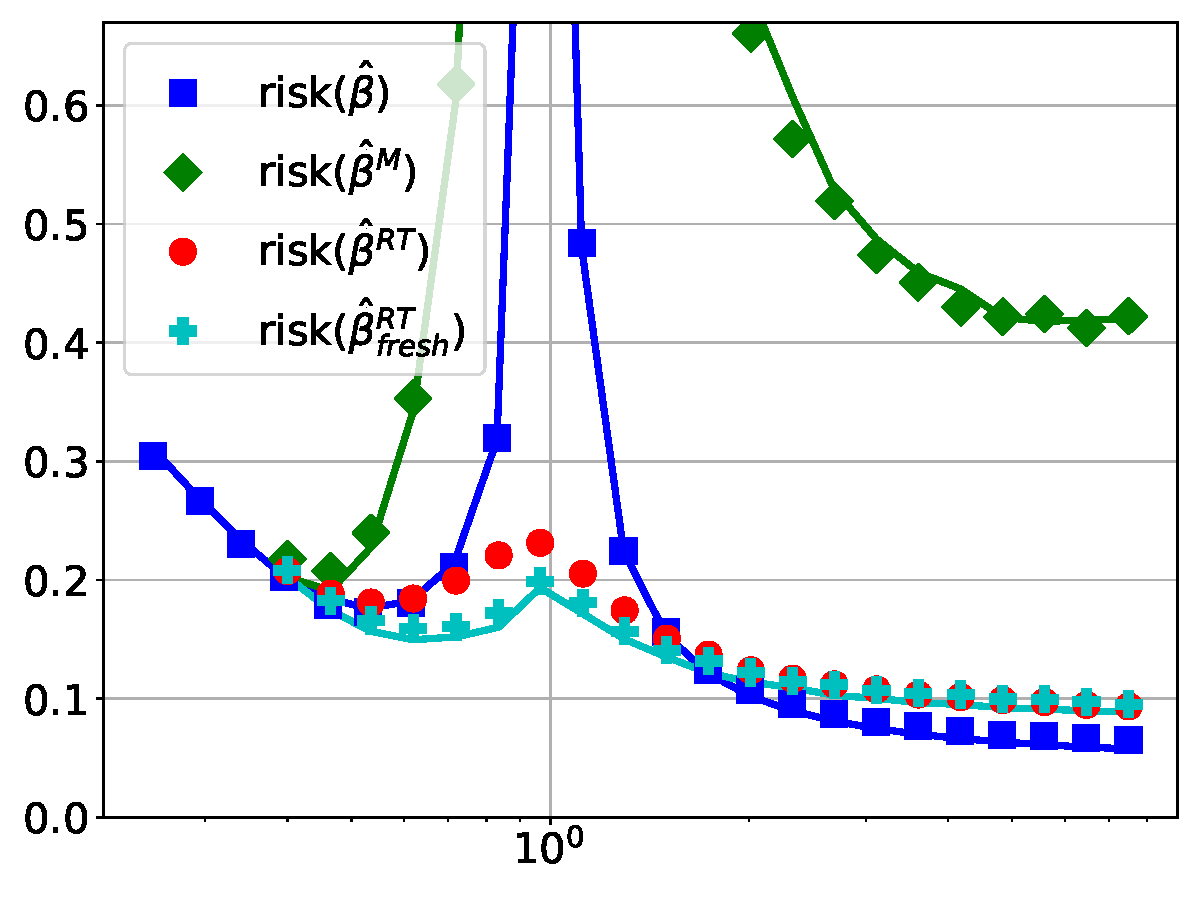
\includegraphics[scale=0.28]{figs2/RF_4s_80_n200_p1500}};
	\node at (-3.1,0) [rotate=90,scale=1.]{Test Risk};
	\node at (0,-2.2) [scale=.9]{Overparameterization ($p/n$)};%Each bar in the figure shows the correlations' geometric mean of datasets in this group when training to corresponding non-zero level. 
	\end{tikzpicture}
	\vspace{-10pt}
	\caption{\small{Illustration of the mismatch between pruning with retraining (red markers) and pruning with fresh samples (cyan markers/line). The setting here is exactly the same as in  Fig.~\ref{figRF}, but we only show the case of sparsity $4s$ for which the mismatch is observed. Observe that our analytical predictions accurately capture the risk of retraining with fresh samples. However, we observe a discrepancy with the true risk of retraining (without fresh samples) around the interpolation threshold. Also shown the risk of the original ERM solution before pruning (in blue) and of the magnitude-pruned model (before any retraining).
%	Same setup as Fig.~\ref{figRF} however we restrict our attention to sparsity $4s$. Green curve is pruning without retraining. Cyan curve retrains with independent samples (unlike red curve). This
	}
	}
	\label{figRF2}\vspace{-15pt}
\end{figure}
\subsection{Random Features Regression} We relate an ERM problem \eqref{eq:ERM} with nonlinear map $\phi$ to an equivalent LGP. This will allow us to use our theoretical results about the latter to characterize the properties of the original nonlinear map. We ensure the equivalence by properly setting up the LGP to exhibit similar second order statistics as the original problem.
\begin{definition}[Equivalent Linear Problem] Given distribution $(\x,y)$ $\sim\Dc$, the equivalent LGP($\bt,\bSi,\sigma$) with $n$ samples is given with parameters $\bSi=\E[\x\x^T]$, $\bt^\st=\bSi^{-1}\E[y\x]$ and $\sigma=\E[(y-\x^T\bt^\st)^2]^{1/2}$. 
\end{definition}
%from equivalent LGP to the original problem  %It should be emphasized that it is important
In Section \ref{sec main}, we formalize the DC of LGPs, which enables us to characterize pruning/retraining dynamics. Then, we empirically verify that DC and pruning dynamics of equivalent LGPs can successfully predict the original problem \eqref{eq:ERM} with non-linear features. The idea of setting up and studying equivalent LGPs as a proxy to nonlinear models, has been recently used in the emerging literature of high-dimensional learning, for predicting the performance of the original ERM task \cite{montanari2019generalization,goldt2020gaussian,abbasi2019universality,derezinski2019exact}. This work goes beyond prior art, which focuses on ERM, by demonstrating that we can also successfully predict the pruning/retraining dynamics. Formalizing the performance equivalence between LGP and equivalent problem is an important future research avenue and it can presumably be accomplished by building on the recent high-dimensional universality results such as \cite{oymak2018universality,hu2020universality,abbasi2019universality,goldt2020gaussian}.


In Fig. \ref{figRF}, we study random feature regression to approximate a synthetic nonlinear distribution. Specifically, data has the following distribution: Given input $\ab\sim\Nn(0,\Iden_d)$, we generate random unit norm $\bt^1\in\R^d,\bt^2\in\R^d$ and set the label to be a quadratic function given by $y=\ab^T\bt^1+(\ab^T\bt^2)^2$. Then, we fix $\Rb\distas\Nn(0,1)$ and we generate ReLU features $\x=\text{ReLU}(\Rb\ab)$, where $\Rb$ corresponds to the input layer of a two-layer network. The markers in Fig. \ref{figRF} are obtained by solving RFR and pruning and retraining with varying sparsity targets ($s,2s,4s$ with $s/n=10\%$). Here, $d=10, n=200$. For each marker, the results are averages of 50 $\Rb\in\R^{p\times d}$ realizations and 10 iterations for each choice of $\Rb$. The lines are obtained via our DC of the equivalent LGP (by using Defs.~\ref{aux_def} and \ref{RT_def}) where the latent parameter $\bt^\st$, noise $\sigma$ and the covariance $\bSi$ of the RFR problem are calculated for fixed realization of the input layer $\Rb$ (similarly averaged over 50 random $\Rb$). Our theory and empirical curves exhibit a good match. The results demonstrate the importance of overparameterization for RF pruning, which corresponds to picking {\em{random features smartly}}. Here, the coefficients of least-squares act like a scoring function for the saliency of random features and capture how well they are aligned with the target function. The fact that the risk of the pruned models is minimized in the overparameterized regime implies that least-squares regression succeeds in properly selecting salient random features from a larger candidate set. In the context of deep learning, our discussion can be interpreted as {\em{pruning hidden nodes of the network}}.

\noindent\textbf{Predicting retraining performance.} As discussed in Sec.~\ref{sec main} and Def.~\ref{RT_def}, for the retraining stage, our DC is accomplished by assuming that retraining phase uses $n$ fresh training examples (i.e.~a new dataset $\Sc_{\text{fresh}}$). Let us denote the resulting model by $\bth^{RT}_{\text{fresh}}$. Perhaps surprisingly, Fig.~\ref{figRF} shows that this DC correctly captures the performance of $\bth^{RT}$ with the exception of the red curve ($4s$). Fig.~\ref{figRF2} focuses on this instance and shows that our DC indeed perfectly predicts the fresh retraining performance and verifies the slight empirical mismatch between $\bth^{RT}$ and $\bth^{RT}_{\text{fresh}}$.
\vspace{-6pt}
\subsection{Neural Network Experiments}\label{ssec:NNE}
Finally, we study pruning deep neural networks.
 %to see the pruning performance under complex models. 
Inspired by  \cite{nakkiran2019deep}, we train ResNet-20 with changeable filters over CIFAR-10. Here, the filter number $k$ is equivalent to the width/channel of the model. As the width of ResNet-20 changes, the fitting performance of the dataset varies. Here, we apply {\em{train$\rightarrow$prune$\rightarrow$retrain}}.
%, since neural networks behave approximately to random feature regression where retraining is crucial to maintain the performance. 
Select $s$ as the sparsity target and $s$-filter ResNet-20 model as the base model with $N_s$ parameters. First, we train a dense model with $k$ filters and $N_k$ parameters, $N_k\gg N_s$, and prune it by only keeping the largest $N_s$ entries in absolute value non-zero. $N_k$ grows approximately quadratically in $k$. Now, the sparse model shares the same number of parameters amenable to training as the base model. Finally, we retain the pruned network and record its performance on the same dataset and same configuration. 
In Fig.~\ref{figNN}, we plot the training and test errors of dense and sparse models. All the neural experiments are trained with Adam optimization and $0.001$ learning rate for $1000$ epochs, with data augmentation. Green, yellow and red lines correspond to $5$, $8$ or $10$ sparsity targets, with around 28,000, 70,000 and 109,000 trainable parameters, respectively. As the width $k$ grows, the training and test errors decrease for all $5$-,$8$-,$10$-filter base models, except for the shaded double descent range. These experiments again verify the main insight revealed to us by studying simpler linear and random-feature models, that is, training a larger model, followed by appropriate pruning, can preform better than training a small model from the beginning.
%
%Our initial argument is proved in neural network experiments that pruning a larger model and pruning could preform better than training a small model from from the beginning. 
Another worth-mentioning observation is that with appropriate sparsity level (here, $10$) the pruned model has prediction performance comparable to the dense model. Finally and interestingly, the test error dynamics of the pruned model exhibit a double descent that resembles that of the dense model (previously observed in \cite{nakkiran2019deep}). 
%More, there is similar double descent behavior in training sparse model as dense model. 



%\newpage